%%%%%%%%%%%%%%%%%%%%%%%%%%%%%%%%%%%%%%%%%
% Short Sectioned Assignment
% LaTeX Template
% Version 1.0 (5/5/12)
%
% This template has been downloaded from:
% http://www.LaTeXTemplates.com
%
% Original author:
% Frits Wenneker (http://www.howtotex.com)
%
% License:
% CC BY-NC-SA 3.0 (http://creativecommons.org/licenses/by-nc-sa/3.0/)
%
%%%%%%%%%%%%%%%%%%%%%%%%%%%%%%%%%%%%%%%%%

%----------------------------------------------------------------------------------------
%	PACKAGES AND OTHER DOCUMENT CONFIGURATIONS
%----------------------------------------------------------------------------------------

\documentclass[paper=a4, fontsize=11pt]{scrartcl} % A4 paper and 11pt font size

\usepackage[T1]{fontenc} % Use 8-bit encoding that has 256 glyphs
%\usepackage{fourier} % Use the Adobe Utopia font for the document - comment this line to return to the LaTeX default
\usepackage[english]{babel} % English language/hyphenation
\usepackage{amsmath,amsfonts,amsthm} % Math packages
\usepackage[utf8]{inputenc}
\usepackage{graphicx}
\usepackage{float}
\usepackage{placeins}
\usepackage[margin=0.8in]{geometry}
\usepackage{mathtools}
\usepackage[]{algorithm2e}
\usepackage{hyperref}
\usepackage{setspace}
\usepackage{booktabs}
\usepackage[table]{xcolor}
\usepackage[T1]{fontenc}
\usepackage[utf8]{inputenc}
\usepackage{tabularx,ragged2e,booktabs,caption}
\usepackage{wrapfig}

\usepackage{caption}
\usepackage{subcaption}
%\usepackage[style=verbose-trad2,natbib=true]{biblatex}
%\usepackage{natbib}
%\usepackage[round, comma, sort&compress]{natbib}
\usepackage{lipsum} % Used for inserting dummy 'Lorem ipsum' text into the template

\usepackage{sectsty} % Allows customizing section commands
\allsectionsfont{\centering \normalfont\scshape} % Make all sections centered, the default font and small caps

\usepackage{fancyhdr} % Custom headers and footers
\usepackage{framed}

\usepackage{listings} % Required for inserting code snippets
%\usepackage[usenames,dvipsnames]{color} % Required for specifying custom colors and referring to colors by name

\definecolor{DarkGreen}{rgb}{0.0,0.4,0.0} % Comment color
\definecolor{highlight}{RGB}{255,255,255} % Code highlight color

\lstdefinestyle{Style1}{ % Define a style for your code snippet, multiple definitions can be made if, for example, you wish to insert multiple code snippets using different programming languages into one document
language=Python, % Detects keywords, comments, strings, functions, etc for the language specified
backgroundcolor=\color{highlight}, % Set the background color for the snippet - useful for highlighting
basicstyle=\footnotesize\ttfamily, % The default font size and style of the code
breakatwhitespace=false, % If true, only allows line breaks at white space
breaklines=true, % Automatic line breaking (prevents code from protruding outside the box)
captionpos=t, % Sets the caption position: b for bottom; t for top
commentstyle=\usefont{T1}{pcr}{m}{sl}\color{DarkGreen}, % Style of comments within the code - dark green courier font
deletekeywords={}, % If you want to delete any keywords from the current language separate them by commas
%escapeinside={\%}, % This allows you to escape to LaTeX using the character in the bracket
firstnumber=1, % Line numbers begin at line 1
frame=single, % Frame around the code box, value can be: none, leftline, topline, bottomline, lines, single, shadowbox
frameround=tttt, % Rounds the corners of the frame for the top left, top right, bottom left and bottom right positions
keywordstyle=\color{Blue}\bf, % Functions are bold and blue
morekeywords={}, % Add any functions no included by default here separated by commas
numbers=left, % Location of line numbers, can take the values of: none, left, right
numbersep=10pt, % Distance of line numbers from the code box
numberstyle=\tiny\color{Gray}, % Style used for line numbers
rulecolor=\color{black}, % Frame border color
showstringspaces=false, % Don't put marks in string spaces
showtabs=false, % Display tabs in the code as lines
stepnumber=5, % The step distance between line numbers, i.e. how often will lines be numbered
stringstyle=\color{Purple}, % Strings are purple
tabsize=2, % Number of spaces per tab in the code
}

% Create a command to cleanly insert a snippet with the style above anywhere in the document
\newcommand{\insertcode}[2]{\begin{itemize}\item[]\lstinputlisting[caption=#2,label=#1,style=Style1]{#1}\end{itemize}} % The first argument is the script location/filename and the second is a caption for the listing

% Image boxes
\newcommand{\subf}[2]{%
  {\small\begin{tabular}[t]{@{}c@{}}
  #1\\#2
  \end{tabular}}%
}


\pagestyle{fancyplain} % Makes all pages in the document conform to the custom headers and footers
\fancyhead[L]{Lars Hertel} % No page header - if you want one, create it in the same way as the footers below
\fancyhead[R]{Data Analysis Report}
\fancyfoot[L]{STATS255} % Empty left footer
\fancyfoot[C]{} % Empty center footer
\fancyfoot[R]{\thepage} % Page numbering for right footer
\renewcommand{\headrulewidth}{1pt} % Remove header underlines
\renewcommand{\footrulewidth}{0pt} % Remove footer underlines
\setlength{\headheight}{13.6pt} % Customize the height of the header

\numberwithin{equation}{section} % Number equations within sections (i.e. 1.1, 1.2, 2.1, 2.2 instead of 1, 2, 3, 4)
\numberwithin{figure}{section} % Number figures within sections (i.e. 1.1, 1.2, 2.1, 2.2 instead of 1, 2, 3, 4)
\numberwithin{table}{section} % Number tables within sections (i.e. 1.1, 1.2, 2.1, 2.2 instead of 1, 2, 3, 4)

\setlength\parindent{0pt} % Removes all indentation from paragraphs - comment this line for an assignment with lots of text

%----------------------------------------------------------------------------------------
%	TITLE SECTION
%----------------------------------------------------------------------------------------

\newcommand{\horrule}[1]{\rule{\linewidth}{#1}} % Create horizontal rule command with 1 argument of height

\title{	
\normalfont \normalsize 
\textsc{University of California, Irvine} \\ [25pt] % Your university, school and/or department name(s)
\horrule{0.5pt} \\[0.4cm] % Thin top horizontal rule
\huge Serum Albumin Analysis\\ % The assignment title
\horrule{2pt} \\[0.5cm] % Thick bottom horizontal rule
}

\author{Lars Hertel,
	ID: 61885853\\} % Your name


\date{\normalsize\today} % Today's date or a custom date

\begin{document}

\maketitle % Print the title

\begin{abstract}
This study attempts to quantify the association of serum albumin and the risk of mortality in end stage renal disease (ESRD) patients. Our inference is based on observational study data from the United States Renal Data System. Specifically, data was collected for patients undergoing hemodialysis in December 2014. We focus on serum albumin at recruitment time and follow up measurements for up to one year after beginning of the study. We consider two categories of models. The first category using serum albumin at baseline and the second utilizing all follow up measurements of serum albumin. Within each category we fit one model with a single serum albumin effect and one letting the effect vary for patients with history of cardiovascular disease (CVD). Using serum albumin at baseline we estimate a 48\% decrease in risk of death for a one g/dL increase in serum albumin. Letting the effect vary for CVD did not produce a statistically significant difference. If we use follow up measurements the estimated effect of serum albumin is a 52\% decrease in risk of death. Differentiating between patients with and without CVD the decrease is 70\% among patients without CVD and 45\% for affected patients.
\end{abstract}

\section{Introduction}
This study is concerned with the effect of protein-energy malnutrition, specifically its marker serum albumin on the mortality of hemodialysis patients. Hemodialysis is a treatment for individuals with end stage renal disease (ESRD). ESRD patient's kidneys are no longer able to filter blood to the extent that is needed by the body. Hence ESRD patients need to have their blood filtered through hemodialysis while they wait for a kidney transplant.
It has been hypothesized that protein-energy malnutrition (PEM) has an effect on mortality among hemodialysis patients. Since serum albumin level can be seen as an indicator of nutritional status or PEM we are interested in the isolated effect of serum albumin on mortality.
%To hypothesize that serum albumin may be related to death makes sense since low albumin may be caused by bad dialyzing. Serum albumin levels are said to be related to cardiovascular disease which is one of the major risks of death among hemodialysis patients.
Serum albumin levels are also impacted by cardiovascular disease (CVD) and its predictors. Since cardiovascular causes account for a large number of deaths among hemodialysis patients \cite{sukhuja} we also want to investigate an effect that depends on the patient's cardiovascular status. Finally, we consider serum albumin to vary over time and test its effect on mortality. We also consider letting the time varying serum albumin levels interact with the cardiovascular disease status. We compare these results to those reported from the analysis based only on one serum albumin measurement.
One of the motivating factors for this study is that if serum albumin was established as an indicator of mortality among hemodialysis patients it would provide an extra criterion for nephrologists to monitor.

\section{Methods}
\subsection{(a)}
We base our analysis on data from the United States Renal Data System (USRDS). This is a data base on patients affected by ESRD in the US. Specifically, patients are included once they survive 90 days on treatment \cite{dan}.

% Describing Sample
The sample is from an observational study of 1,979 hemodialysis patients. We sample from all patients that were undergoing dialysis in December 2014. That means both patients that just started dialysis and patients that had been on the treatment for a long time can enter the study. We draw the sample from dialysis clinics across the US. Measurements are taken at the time of recruitment. These include the serum albumin level, demographics and lab measurements. In order to quantify the time-varying effect of serum albumin followup measurements were also taken. These are at intervals of 1 to 2 months for up to one year after the first measurement.

% Introduce variables and Missingness
The data set includes 15 variables that were recorded. We note that the sample has missing values across different variables. We will describe this in detail in section \ref{sec:results_a} of the report. The measured variables are the time in days from recruitment to the end of observation and whether the individual died at the end of this time period. We also have the patients age in years at recruitment, their gender, race group (caucausian, African American or other), their smoking status at the time of first access placement (never smoked, former smoker or current smoker). We have indicators of whether the patient has a history of cardiovascular disease, has diabetes (type I or II) and how long they had ESRD prior to the study. The nurse recorded whether the patient appeared undernourished at recruitment and their body mass index as weight(kg) divided by height(m) squared. Finally, measurements were taken of the patient's serum albumin level (g/dL), total serum cholesterol (mg/dL), serum triglycerides (mg/dL) and post dialysis blood pressure (mmHg) all at time of recruitment. Finally we have follow up measurements of serum albumin (g/dL) along with the time in days between start of the study and measurement.



\subsection{(b)}
\label{sec:methods_b}

% Describe Cox Model
Throughout this study we will use a proportional hazards model to compare the hazard across sub-populations. This means that while the hazard itself is allowed to change over time, we assume that the hazard ratio between sub-populations remains constant. We further attempt to model this hazard ratio as the exponential of a linear combination of predictor variables. This is considered a semi-parametric approach. While we impose a parametric form on the hazard ratio we do not model the baseline hazard itself. We thus restrict ourselves to the comparison of sub-populations with this model. We further make the assumption that censoring happens independently of death, the event of interest.
We expect that main reasons for censoring are failure to follow up and receiving a transplant. We assume that the independence assumption is valid.\\
% How does censoring come about in this study?
% Transplant
% End of study

% Interpretation
We interpret coefficients in the Cox model in terms of their exponentiated transformations which yield the adjusted relative risk (aRR). For an indicator of a feature the exponentiated coefficient represents the adjusted relative risk of the event (here death) of the group with the feature as compared to without the feature. For continuous variables the exponentiated coefficient represent the adjusted relative risk comparing a subpopulation with a one unit higher value in the variable than another.\\

% Describe Time varying modelling
Aside from quantifying the effect of the baseline serum albumin level we are also interested in the time varying effect. Serum albumin levels are expected to vary over time for hemodialysis patients. For this reason we consider follow-up data in which serum albumin was measured in 1 to 2 month intervals. Thus we would like to model this change in serum albumin for each subject as they move through time. In that sense we simply update each patient's value of serum albumin as it changes.\\ %In this scenario we cannot factor out the baseline hazard anymore as explained above.
% Comment?!?!?!?!

%% Model building
% Intro
In our model building we want to adjust for two types of risk factors: those that confound the relationship between serum albumin and mortality and those that are independently of serum albumin predictors of mortality. We refer to the former as confounding variables and the latter as precision variables.\\

% Philosophy
We build our model before considering the data set in order to achieve maximal generalizability of our results. The motivation behind this is that drawing on general scientific results in the variable selection will make our model more robust to spurious effects in the sample. In that manner we will first consider general factors of mortality in hemodialysis patients. We will then decide which work as confounding variables and which as precision variables dependent on whether they have an association with serum albumin. Finally, we will match these factors to variables in our data set.\\

% Factors of Mortality in Hemodialysis patients
According to \cite{elsharif}, \cite{mailloux} and \cite{sukhuja} the main causes of death among hemodialysis patients are related to infection, cardiac causes or withdrawal. Especially \cite{mailloux} states that during the first 4 years of treatment the former two causes mainly govern mortality. Note that \cite{elsharif} refers to a study conducted outside of the US.\\

% Cardiac causes
We decide that factors of cardiac issues are diet, obesity, gender, lack of exercise, history of cardiovascular disease, smoking, high systolic blood pressure and high cholesterol \cite{uptodate}. We further decide that diabetes may be a predictor of obesity, lack of exercise and high blood pressure. Among these factors we have matching measurements in the data set of body mass index (obesity), gender, history of cardiovascular disease, smoking group, post dialysis systolic blood pressure, cholesterol and diabetes.\\

% Infection
Furthermore, we consider predictors of infection. We decide that infection is generally provoked by weakness in the body. Thus we understand that an individuals diet, lack of exercise, smoking behaviour and time on dialysis may make him/her prone to infection. In addition, diabetes patients are at increased risk of infection. Finally, we note that hemodialysis patients are at increased risk of infection through the dialysis access. Matching variables in the data set are an indictor of under nourishment, smoking group, time on dialysis and diabetes.\\

We also decide that time on dialysis may be related to depletion of serum albumin. It is therefore a potential confounder of the relationship of interest. We decide that under nourishment is closely related to serum albumin because serum albumin is a biomarker of nutritional level. We decide not to include under nourishment in the model since it may be part of the effect we are trying to isolate. We do not decide on any effect modifiers in the relationship between serum albumin and mortality apart from history of CVD.\\
We want to note that we lack information about the access type that dialysis is conducted with.

% Comments
%We note that we lack a variable that reliably represents a patient's diet.

\section{Results}
\subsection{(a)}
\label{sec:results_a}
% EDA
% Time in Study
We consider descriptive statistics of each of our measured variables. We can see from table \ref{tab:cat} that approximately a quarter of the subjects experience death during study time. The mean time in the study of 366.8 is not very significant since the distribution is highly skewed as can be seen in figure \ref{fig:timeinstudy_hist}. Most subjects stay to the end of the study and get censored. If we consider the distribution of time in study conditional upon experiencing death (\ref{fig:timeinstudy_hist} right) we can see there is a large amount of people who die soon after enrollment. After that subjects seem to die uniformly across time. Since subjects are enrolled having been on hemodialysis for different amounts of time this is difficult to interpret. We thus consider the time from ESRD diagnosis to death for subjects that died in figure \ref{fig:esrdtimetilldeath_hist}. This seems to follow a roughly exponential form with half of the subjects dying within two years.

\begin{figure}[H]
\centering
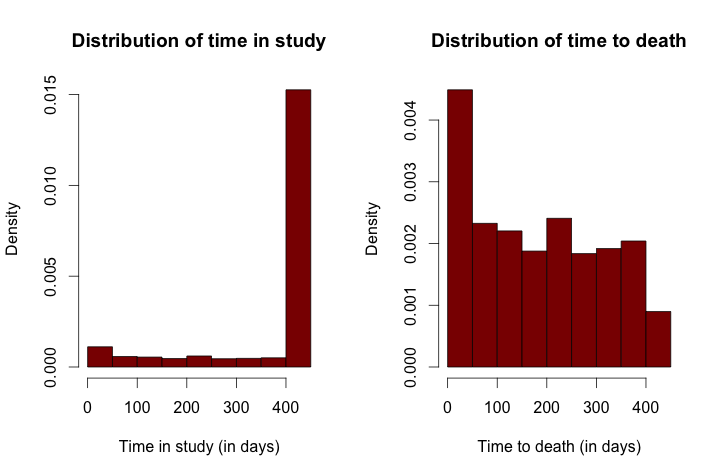
\includegraphics[width=0.7\textwidth]{plots/timeinstudy_hist.png}
\caption{Distributions of time in study for all subjects (left) and for subjects that experience death (right).}
\label{fig:timeinstudy_hist}
\end{figure}

\begin{figure}[H]
\centering
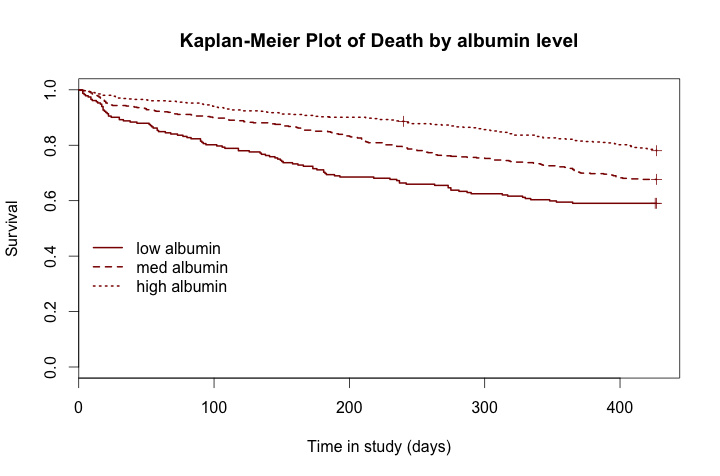
\includegraphics[width=0.7\textwidth]{plots/death_km.png}
\caption{We show a plot of survival grouping subjects into albumin levels given by the 33rd and 66th quantiles. It can be seen that survival decreases for the medium and low albumin groups.}
\label{fig:death_km}
\end{figure}


\begin{table}[ht]
\centering
\begin{tabular}{rll}
  \hline
 & median (SD) & Number of NAs \\ 
  \hline
tdeath & 427(123.19) & 0 \\ 
  age & 63(15.35) & 0 \\ 
  esrdtime & 1.8(3.52) & 0 \\ 
  bmi & 23.73(5.76) & 41 \\ 
  albumin.0 & 3.8(0.5) & 0 \\ 
  cholest & 170(49.58) & 147 \\ 
  trigly & 140(139.95) & 392 \\ 
  pst.sbp & 134(21.55) & 32 \\ 
   \hline
\end{tabular}
\caption{Summary measures of the continuous variables in the dataset. We also indicate the number of missing values in each variable.}
\label{tab:cont}
\end{table}

% Continuous variables
Distributions of the continuous variables are shown in figure \ref{fig:cont_box}. Furthermore, we show summary statistics of the continuous variables in table \ref{tab:cont}. Age is skewed with fewer subjects at a very young age. The median age is at 63. The ESRD time prior to the study is right skewed with 75\% lying between 0 and 5 years. This is in line with the distribution of time on ESRD for subjects that die or not die which we considered in \ref{fig:esrdtimetilldeath_hist}. The distribution of BMIs symmetrical about the median of 23.73 with outliers of high BMIs. A similar distribution can be seen for cholesterol. Post dialysis systolic blood pressure seems to be slightly elevated at median 135 (compared to the ideal 90-120 mmHg). The distribution seems symmetric with few high and low outliers. We also show plots of the continuous variables against one another in figure \ref{fig:pairs}. No clear association is indicated.

\begin{figure}[H]
\centering
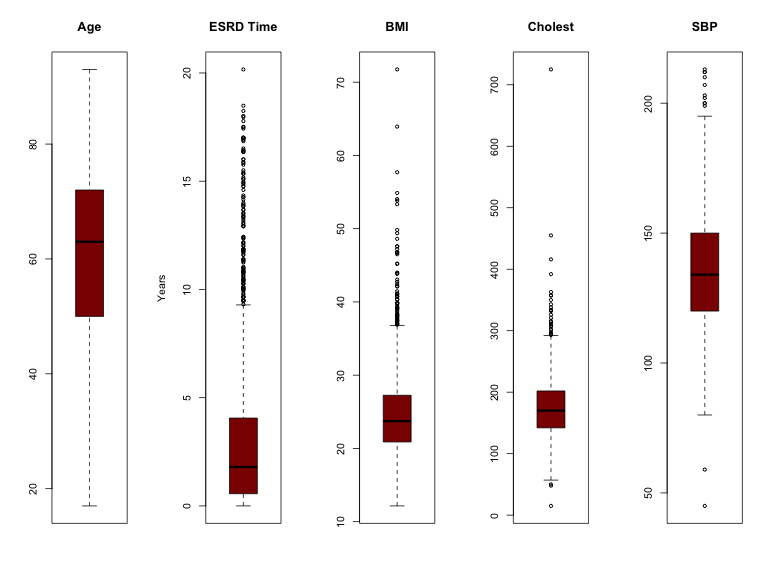
\includegraphics[width=.6\textwidth]{plots/cont_box.png}
\caption{Distributions of continuous variables.}
\label{fig:cont_box}
\end{figure}

% Serum albumin
Serum albumin, the variable of interest shows a roughly bell-shaped distribution around the median of 3.8 as shown in figure \ref{fig:albumin_hist}. We also show how the distribution of serum albumin changes when we stratify by the different variables in the dataset (figure \ref{fig:albumin_biv_box}). The most significant difference in distributions is shown when we stratify by under nourishment. This makes sense since we expect serum albumin to be a marker of nutritional status.

\begin{figure}[H]
\centering
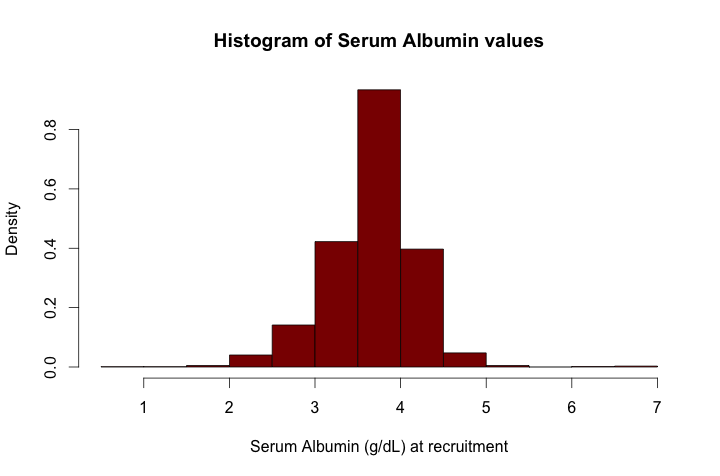
\includegraphics[width=.6\textwidth]{plots/albumin_hist.png}
\caption{Distributions of continuous variables.}
\label{fig:albumin_hist}
\end{figure}

% Categorical variables
We now consider the categorical variables that we have recorded in the data set. For this we mainly consider table \ref{tab:cat}. We have a balanced data set of almost equal halfs women and men. It is made up of mainly whites and African Americans. It is surprising that less than 10\% are from other races. Specifically we would expect hispanics and asians to take a larger part in the study. This may be due to the locations that the data had been taken from. If this is not the case this would pose the question whether caucasians and African American's are at higher risk of ESRD. There are 30 subjects in the study that we do not have race information for.
The majority of subjects in the study classify themselves as having never smoked. 

\begin{table}[H]
\centering
\begin{tabular}{rll}
  \hline
 & count (proportion) & Number NAs \\ 
  \hline
death & 490(25\%) & 0 \\ 
  female & 966(49\%) & 0 \\ 
  racegrp & --- & 30 \\ 
  caucasian & 1033(53\%) & --- \\ 
  african & 766(39.3\%) & --- \\ 
  other & 150(7.7\%) & --- \\ 
  smokegrp & --- & 177 \\ 
  never smoked & 999(55.44\%) & --- \\ 
  former smoker & 527(29.25\%) & --- \\ 
  current smoker & 276(15.32\%) & --- \\ 
  hist.cvd & 1080(59\%) & 161 \\ 
  diabetes & 710(36\%) & 9 \\ 
  undnour & 344(19\%) & 120 \\ 
   \hline
\end{tabular}
\caption{Descriptive statistics for categorical variables in the dataset.}
\label{tab:cat}
\end{table}

% Categorical variables continued
Considering that 75\% of the subjects are 50 years or older and smoking rates in the 60s and 70s used to be 40\% \cite{gallup} we would expect at least 30\% to have smoked before. Information on smoking is missing for 177 subjects. Due to the nature of the variable this could be a case of non-ignorable missingness since current smokers might be more hesitant to report their status than people who do not smoke.
Next, we consider the proportion of people who have history of cardiovascular disease. This is at 59\% with 161 subjects missing. This is not surprising. In fact we have 70\% of subjects between 60 and 80 years of age with a history of cardiovascular disease which exactly corresponds to the estimated proportion in the population given by \cite{cvd}. However, proportions among 20 to 40 year old and 40 to 60 year old are approximately 100\% and 50\% higher in our sample than in \cite{cvd}, while proportions for over 80 year olds are 30\% lower.
We note that smoking status and history of CVD tend to be missing together in the data set as shown in figure \ref{fig:na_pattern}.\\ % more on pattern

We have a rate of diabetes at 36\% in the sample with 9 subjects missing information. This is a almost 300\% higher rate than in the overall population (9.3\% according to American Diabetes Association\cite{ADA}). The higher rate is expected since diabetes is a cause of ESRD. In addition, the age distribution in the sample is higher than in the overall population. We were not able to find a comparison for diabetes rates among ESRD patients. \\

Finally, we consider under nourishment in our sample. We have 344 subjects (19\%) that were classified as under nourished. Note however that 120 subjects are missing information. At worst all these subjects were under nourished which could seriously impact the results. It is possible that the missing cases are where the nurse found it difficult to decide on their status. In that case we might miss borderline cases which would be less severe. However, we cannot say for certain how the missingness came about and it might be critical for this variable. We show an overview of missingness in figure \ref{fig:na_pattern}.\\

% Missingness
We can see that smoking status and CVD history tend to be missing together as mentioned above. Furthermore, under nourishment tends to miss together with these variables. Finally, cholesterol and triglycerin tend to miss together. Especially, triglycerin has a large number of missing values (392). Since we expect history of CVD to be a strong predictor of death among hemodialysis patients we investigate its missingness in more detail (see figure \ref{fig:hist_na})



\begin{figure}[H]
\centering
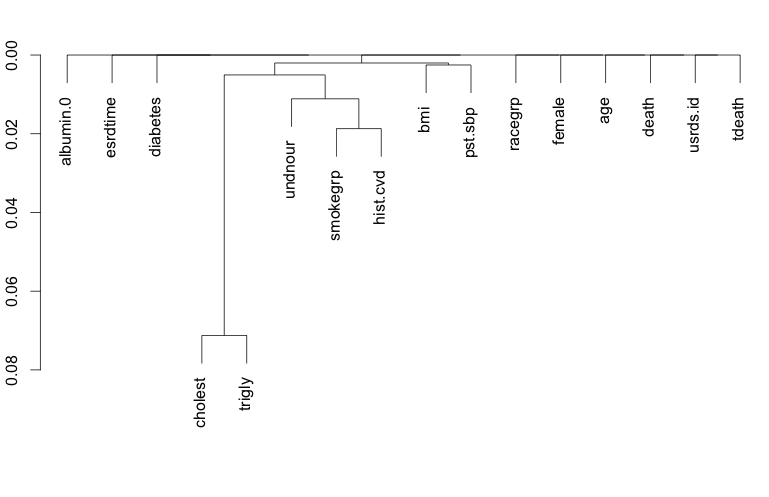
\includegraphics[width=.6\textwidth]{plots/na_pattern.png}
\caption{Diagram showing patterns of which variables tend to be missing simultaneously in the data set.}
\label{fig:na_pattern}
\end{figure}







\subsection{(B)}
% Intro
Throughout this section we will present the three major models in this study. We decided on the adjustment variables a priori in section \ref{sec:methods_b}. We will refer to the three models as A, B, C and D. Model A includes serum albumin only as a main effect. Model B allows the effect of serum albumin on mortality to change by history of CVD. Model C allows for the serum albumin level of a subject to change over time. Model D incorporates a time varying serum albumin level and allows for the effect to be different for subjects with and without history of CVD. Note that we described missingness in the previous section. We will for this section rely on a complete case analysis of the data.

% Model A
Table \ref{tab:model_a} shows the adjusted relative risk (aRR) of death by patient characteristics. For more information on aRR see section \ref{sec:methods_b}. Adjustment was done by under nourishment, time on ESRD, BMI, smoking status, cholesterol level, diabetes status, post-dialysis systolic blood pressure, gender, age and history of CVD. The aRR of serum albumin was lower with increasing serum albumin levels (aRR = 0.52, 95\% CI: 0.42, 0.65, p < 0.001). An increase in Body Mass Index was associated with a decreased risk (aRR = 0.96, 95\% CI: 0.94, 0.98, p = 0.003). Being a current smoker compared to having never smoked as a higher aRR (aRR = 1.59, 95\% CI: 1.17, 2.16, p = 0.003). Age yielded a statistically significant increase in aRR (aRR = 1.04, 95\% CI: 1.03, 1.04, p < 0.001). That means that for a 10 year increase in age we have a corresponding approximate increase of 34\% in risk. Having a history of CVD also resulted in a higher aRR (aRR = 2.07, 95\% CI: 1.58, 2.71, p < 0.001). Time on ESRD, being a former smoker as compared to having never smoked, cholesterol level, diabetes, post-dialysis systolic blood pressue and gender were not associated with risk of death.

% Diagnostics
We show diagnostic plots in figures \ref{fig:modela_diag} and \ref{fig:modela_dfbeta}. We decide that a log-transform of albumin at recruitment time may be appropriate. We do not find significant outliers or influential points. The proportional hazards assumption seems to be reasonably fulfilled.


\begin{table}[ht]
\centering
\begin{tabular}{rll}
  \hline
 & Adjusted relative risk (95\% CI) & p-Value \\ 
  \hline
albumin.0 & 0.52(0.42 ,0.65) & 0 \\ 
  esrdtime & 0.99(0.96 ,1.03) & 0.661 \\ 
  bmi & 0.96(0.94 ,0.98) & 0.001 \\ 
  factor(smokegrp)2 & 1.01(0.78 ,1.3) & 0.968 \\ 
  factor(smokegrp)3 & 1.59(1.17 ,2.16) & 0.003 \\ 
  cholest & 1(0.99 ,1) & 0.024 \\ 
  diabetes & 1.2(0.95 ,1.5) & 0.12 \\ 
  pst.sbp & 1(0.99 ,1) & 0.067 \\ 
  female & 0.98(0.78 ,1.24) & 0.89 \\ 
  age & 1.04(1.03 ,1.04) & 0 \\ 
  hist.cvd & 2.07(1.58 ,2.71) & 0 \\ 
   \hline
\end{tabular}
\caption{Regression estimates of the adjusted relative risk (aRR) from a Cox proportional hazards model.}
\label{tab:model_a}
\end{table}



% Model B
Model B is identical to model A but allows for the effect of serum albumin to differ between subjects with and without history of CVD. The adjusted relative risks by patient characteristics are shown in table \ref{tab:model_b}. We note that a one g/dL increase in serum albumin is associated with a 43\% decrease in risk for patients without CVD (aRR = 0.37, 95\% CI: 0.25, 0.56, p < 0.001). For patients with CVD this is only a 42\% decrease (aRR = 0.58, 95\% CI: 0.25, 1.39, p = 0.058). At a serum albumin value of 3.5 patients with CVD have an estimated 975\% higher risk of death than patients without. At serum albumin of 4.0 this is increased to a 1246\% higher risk. Here 3.5 and 4.0 correspond to the approximate 33\% and 66\% percentiles in serum albumin measures at baseline. Note that the difference of serum albumin coefficients between CVD and non-CVD is not statistically significant. We assume that we might not have enough observations to estimate the effect with enough precision.
%We estimate a 63\% decrease in aRR associated with an increase of serum album of one g/dL. The effect of history of CVD has become more pronounced (aRR = 2.21, 95\% CI: 1.67, 2.94, p < 0.001). The effect of serum albumin for patients with history of CVD is (aRR = 1.56, 95\% CI: 0.98, 2.49, p = 0.058). We note that this effect is not statistically significant. 
The remaining estimates are equal to those in the model A. We show diagnostic plots in figures \ref{fig:modelb_diag} and \ref{fig:modelb_dfbeta}. We note that there are three points with high influence on the coefficient of history of CVD. We decide to remove these in the post-hoc analysis.\\



% Model C
In model C we allow serum albumin values to vary with time. We use the data collected on follow up measurements on each patient. The estimated aRRs for each patient characteristic are shown in table \ref{tab:model_c}. Compared to model A the overall interpretation stays similar. Serum albumin is estimated to decrease aRR by 52\% for a one g/dL increase (aRR = 0.48, 95\% CI: 0.42, 0.54, p < 0.001). BMI (aRR = 0.95, 95\% CI: 0.94, 0.97, p < 0.001), being a current smoker (aRR = 1.63, 95\% CI: 1.39, 1.91, p < 0.001), age (aRR = 1.03, 95\% CI: 1.03, 1.04, p < 0.001) and history of CVD (aRR = 1.97, 95\% CI: 1.72, 2.26, p < 0.001) have similar effects as in model A. However, diabetes is now also estimated to change the relative risk of death (aRR = 1.15, 95\% CI: 1.02, 1.3, p = 0.02). We note that the confidence interval for serum albumin is smaller as compared to model A (\ref{tab:model_a}). This is likely due to the increased power that the repeated measurements of serum albumin yield in the estimation of the coefficient. %Furthermore, we see model C as a more accurate model since it takes non-proportional hazards over time into account.
We check diagnostics for model C in figure \ref{fig:modelc_diag} and \ref{fig:modelc_dfbeta}. We find similar diagnostics as for model A. We thus decide not to remove any observations but propose a log transform on albumin.\\

% Model D
Model D (table \ref{tab:model_d}) incorporates serum albumin as a time varying covariate and allows for its effect to be different for patients with and without history of CVD. This model indicates a 70\% (aRR = 0.3, 95\% CI: 0.24, 2.53, p < 0.001) decrease in risk of mortality for a one g/dL increase in serum albumin for patients without CVD. For patients with history of CVD it estimates a 45\% decrease (aRR = 0.55, 95\% CI: 0.33, 0.90, p < 0.001). Having a history of CVD increases the risk 17-fold at a serum albumin level of 3.5 and 17.2-fold at 4.0. The effects of BMI, being a current smoker, diabetes, systolic blood pressure after dialysis and age remain similar as in model C. Time on ESRD, being a former smoker, cholesterol and gender do not have an effect on the risk of death. We checked the model diagnostics with similar results as for model C.

\subsection{(C)}
In this section we aim to explore models that are counterparts to our choice of model above or that arose out of findings in the exploratory data analysis.\\

% Model with under nourishment
We had a priori decided not to adjust for under nourishment of a patient. The reasoning behind this was that serum albumin is a marker of nutritional level itself. We reasoned that for the scientific question of interest it is more appropriate to consider serum albumin alone as nutritional marker. We expect a correlation between under nourishment and low serum albumin levels. Adjusting for under nourishment in a patient might take away from the effect that we want to quantify. In figure \ref{fig:albumin_biv_box} we see that the association between serum albumin and under nourishment is mild. For secondary analysis we thus adjust for under nourishment (model E, table \ref{tab:model_e}) using time varying serum albumin without CVD interaction. Note that despite choosing model D as our final model we use the model without interaction here since the coefficients have more intuitive interpretations. We see that as expected under nourishment increases risk of death by an estimated 74\% and albumin is estimated to decrease the risk by 46\% (compared to 52\% in the model without adjustment for under nourishment). History of CVD is estimated to increase the risk by 116\% as compared to 97\% in model C. The remaining estimates stay approximately constant.\\

% Model with sqrt ESRD time
Next, we explored a transformation of the time patients had been dialysing when entering the study. We expected a priori for ESRD time to have an impact on risk of death. However, none of the models presented above showed a statistically significant effect of this covariate. Figure \ref{fig:albumin_hist} shows that ESRD time is right skewed. It is natural to think of a log transformation to linearize this variable. In this case we choose a square-root transformation due to its similarlity to a log-transform and because we have observations with ESRD time zero. We refit model C with square-rooted ESRD time. The square-root transformation does not yield any significant changes in the fit of the model. Square rooted ESRD time is estimated to not have an effect on risk of death.\\

% Model with log albumin
We now consider a model with log-base-2 transformed albumin variable. Again we consider model C as basis and transform albumin accordingly. The resulting model F estimates a 77\% decrease in risk of death for a two-fold increase in serum albumin. In order to compare this to model C we consider an increase from 3.5 to 4.5 g/dL serum albumin. Model C estimates a 52\% decrease in risk for this change. Model F estimates a 41\% decrease in risk of death. The log-transformed model thus seems to be more conservative. The confidence intervals have approximately the same width in both models.

% Removing BMI or cholesterol
Finally, we investigate removing cholesterol or BMI from the model. We decided on both variables a priori as risk factors in hemodialysis patients. Figure \ref{fig:pairs} does not show any dramatic association between the continuous covariates in our dataset. Nevertheless, we consider the effect of removing either covariate. We find that removing BMI causes being a former smoker to have significant effect. This effect is estimated to increase risk by 15\%. It also makes cholesterol significant at a p-value of 0.05. This would cause a risk decrease of 9\% between the 1st quartile of cholesterol (142 mg/dL) and the 3rd quartile (202 mg/dL). Removing cholesterol as variable from the model does not cause significant changes in the estimated effects of the other variables.

% Imputation of missing values

\section{Discussion}
This study gives evidence that in the population of hemodialysis patients in the US those with higher serum albumin values have lower risk of death. If we only consider serum albumin at recruitment a one g/dL higher serum albumin level is associated with an estimated 48\% decrease in risk of death. Letting this effect vary across patients with and without CVD does not produce a statistically significant effect. Using a model that allows for time varying serum albumin though follow up measurements, we quantify this effect as a 52\% decrease in risk of death for a one g/dL increase of serum albumin. If we let patients with CVD have a different effect this is a 70\% decrease for patients without CVD and a 45\% decrease for patients with CVD.

Our study is thus consistent with previous findings (\cite{mutsert}, \cite{kalantar}). The associated increase in risk for a one g/dL decrease in serum albumin is however twice as big in our study as compared to that shown by \cite{mutsert}.\\
% Limitations in sampling scheme
% Ideal sample
We consider limitations in the generalizability of this study. An ideal study would pick a random sample of all dialysis patients across the world. In order to avoid confounding effects one would randomize treatments. In this case, one would randomly assign different values of serum albumin. After blinding and randomization the time to death would be measured. Conducting a randomized experiment with assignment of serum albumin values is practically difficult.\\

The data at hand is thus from an observational study. This means that there is potential for our results to be affected by confounding factors. In other words, at worst we may not be able to isolate the effect of serum albumin and thus falsely quantify it.\\

%% Potential problems with the sample
% Sampling Scheme
Additional issues might arise from the sampling scheme. The data set is left truncated since patients are entered into the data base after 90 day survival on hemodialysis. If there are strong effects of serum albumin on mortality during the initial stages of dialyzing we do not estimate those in our analysis. At worst our results may not be applicable to early stage hemodialysis patients.\\

% Limitations in measured variables
We did not adjust for race in our analysis. The large majority of study participants was caucasian or African-American. It is hence questionable whether Hispanics or Asians entered the study at all (classified as other). This may limit the generalizability of our study in terms of race.\\

% Limitations due to missing data
Finally, we have a substantial amount of missing values in the dataset. The variables with the most impactful amounts of missing data (under nourishment and triglycerin) were not included in the model that we had decided upon a priori. There is however a substantial amount of missing data in CVD history and smoking status. History of CVD is balanced with 59\% of observed subjects having CVD. Among smokers the 177 missing observations could however heavily impact the results if they are all current smokers. This is because the group of current smokers consists of only 276 subjects.


% Generalizability
Overall, we expect to be able to generalize to hemodialysis patients in the US who have survived hemodialysis for 90 days. Nevertheless, we want to treat the results conservatively due to the above mentioned limitations in the study.


\begin{thebibliography}{9}
\bibitem{dan} 
Gillen D., Stehman-Breen C., Smith J., McDonald R., Warady B. Brandt J., and Wong C., “The survival advantage
of pediatric recipients of a first kidney transplant among children awaiting kidney transplantation.” American Journal of
Transplantation, Vol. 8, No. 12 (2008), pp. 2600-6.


\bibitem{kidney}
The National Kidney Foundation
\url{https://www.kidney.org/atoz/content/dialysisinfo}

\bibitem{elsharif}
Elsharif, Mohamed Elhafiz. "Mortality rate of patients with end stage renal disease on regular hemodialysis: A single center study." Saudi Journal of Kidney Diseases and Transplantation 22.3 (2011): 594.

\bibitem{mailloux}
Mailloux, Lionel U., et al. "Mortality in dialysis patients: analysis of the causes of death." American journal of kidney diseases 18.3 (1991): 326-335.

\bibitem{sukhuja}
Sakhuja, Rahul, et al. "End-stage renal disease and sudden cardiac death." Cardiac Electrophysiology Clinics 1.1 (2009): 61-77.

\bibitem{moon}
Wang, Angela Yee-Moon, et al. "Sudden cardiac death in end-stage renal disease patients a 5-year prospective analysis." Hypertension 56.2 (2010): 210-216.

\bibitem{uptodate}
\url{http://www.uptodate.com/contents/estimation-of-cardiovascular-risk-in-an-individual-patient-without-known-cardiovascular-disease}

\bibitem{gallup}
\url{http://www.gallup.com/poll/109048/us-smoking-rate-still-coming-down.aspx}

\bibitem{cvd}
Go, AS; Mozaffarian, D; Roger, VL; Benjamin, EJ; Berry, JD; Borden, WB; Bravata, DM; Dai, S; Ford, ES; Fox, CS; Franco, S; Fullerton, HJ; Gillespie, C; Hailpern, SM; Heit, JA; Howard, VJ; Huffman, MD; Kissela, BM; Kittner, SJ; Lackland, DT; Lichtman, JH; Lisabeth, LD; Magid, D; Marcus, GM; Marelli, A; Matchar, DB; McGuire, DK; Mohler, ER; Moy, CS; Mussolino, ME; Nichol, G; Paynter, NP; Schreiner, PJ; Sorlie, PD; Stein, J; Turan, TN; Virani, SS; Wong, ND; Woo, D; Turner, MB; American Heart Association Statistics Committee and Stroke Statistics, Subcommittee (1 January 2013). "Heart disease and stroke statistics--2013 update: a report from the American Heart Association.". Circulation 127 (1): e6–e245.

\bibitem{ADA}
\url{http://www.diabetes.org/diabetes-basics/statistics/}

\bibitem{mutsert}
de Mutsert, Renée, et al. "Association between serum albumin and mortality in dialysis patients is partly explained by inflammation, and not by malnutrition." Journal of renal nutrition 19.2 (2009): 127-135.

\bibitem{kalantar}
Kalantar-Zadeh, Kamyar, et al. "Revisiting mortality predictability of serum albumin in the dialysis population: time dependency, longitudinal changes and population-attributable fraction." Nephrology Dialysis Transplantation 20.9 (2005): 1880-1888.


 
\end{thebibliography}

\pagebreak

\appendix

\section{Exploratory Data Analysis}

\begin{figure}[H]
\centering
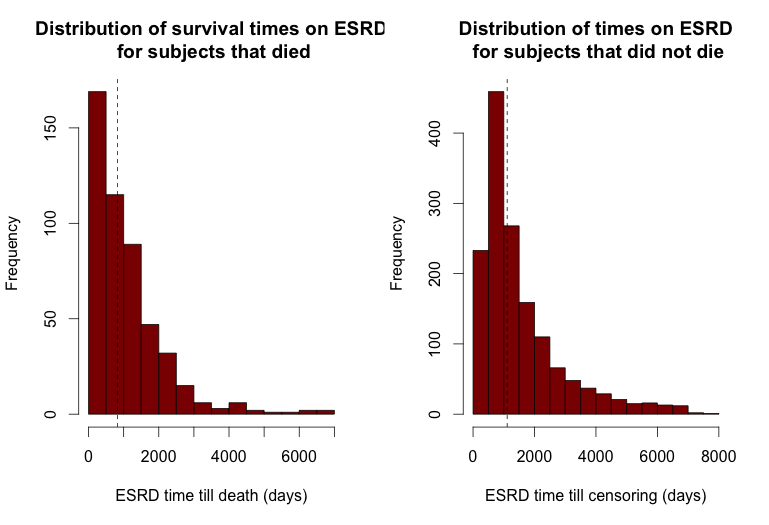
\includegraphics[width=0.7\textwidth]{plots/esrdtimetilldeath_hist.png}
\caption{Distributions of time on ESRD conditioning upon that the subject died. This is the sum of the ESRD time (scaled to days) plus the time to death in the study. The dashed line indicates the median survival time.}
\label{fig:esrdtimetilldeath_hist}
\end{figure}

\begin{figure}[H]
\centering
\caption{Plots of continuous covariates against one another. None of the plots indicates a clear linear association.}
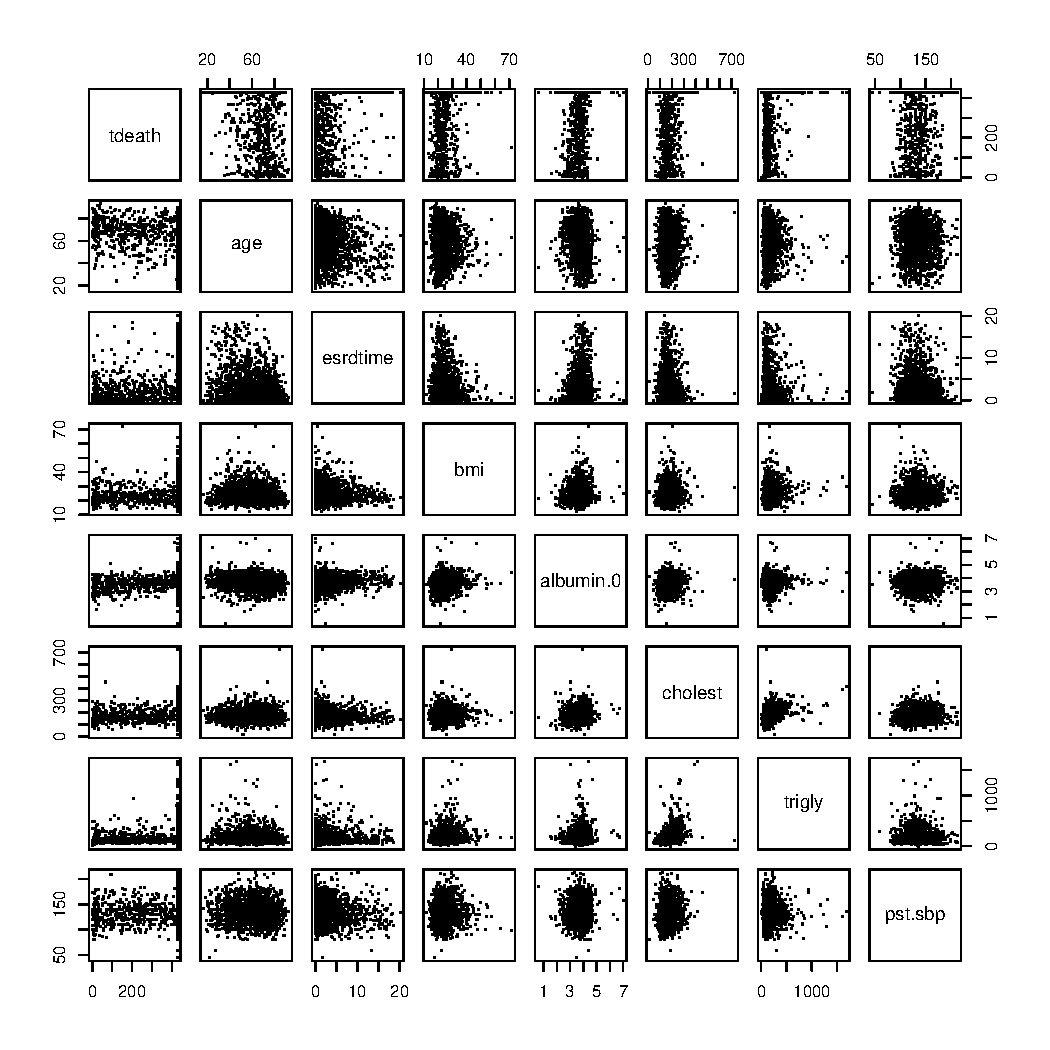
\includegraphics[width=.8\textwidth]{plots/pairs.pdf}
\label{fig:pairs}
\end{figure}


\begin{figure}[H]
\centering
\caption{Distribution of serum albumin levels (y-axis) stratified by the variables in the data set.}
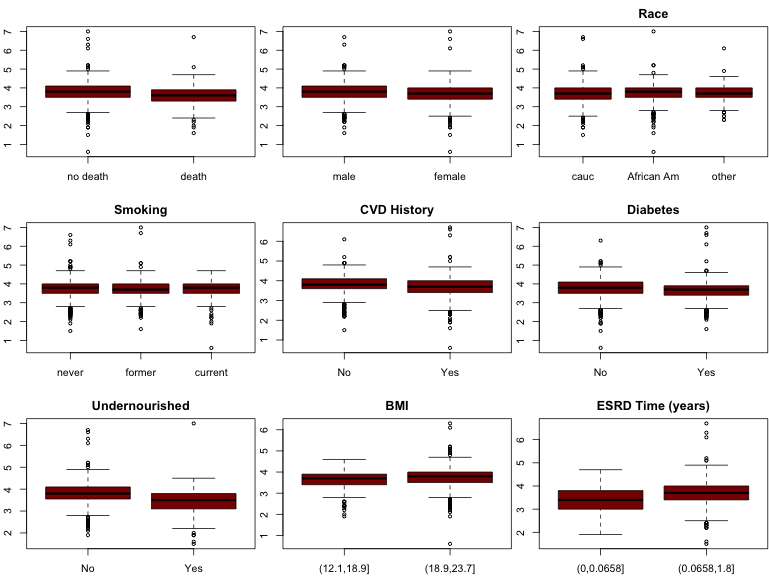
\includegraphics[width=.8\textwidth]{plots/albumin_biv_box.png}
\label{fig:albumin_biv_box}
\end{figure}



\begin{figure}[H]
\centering
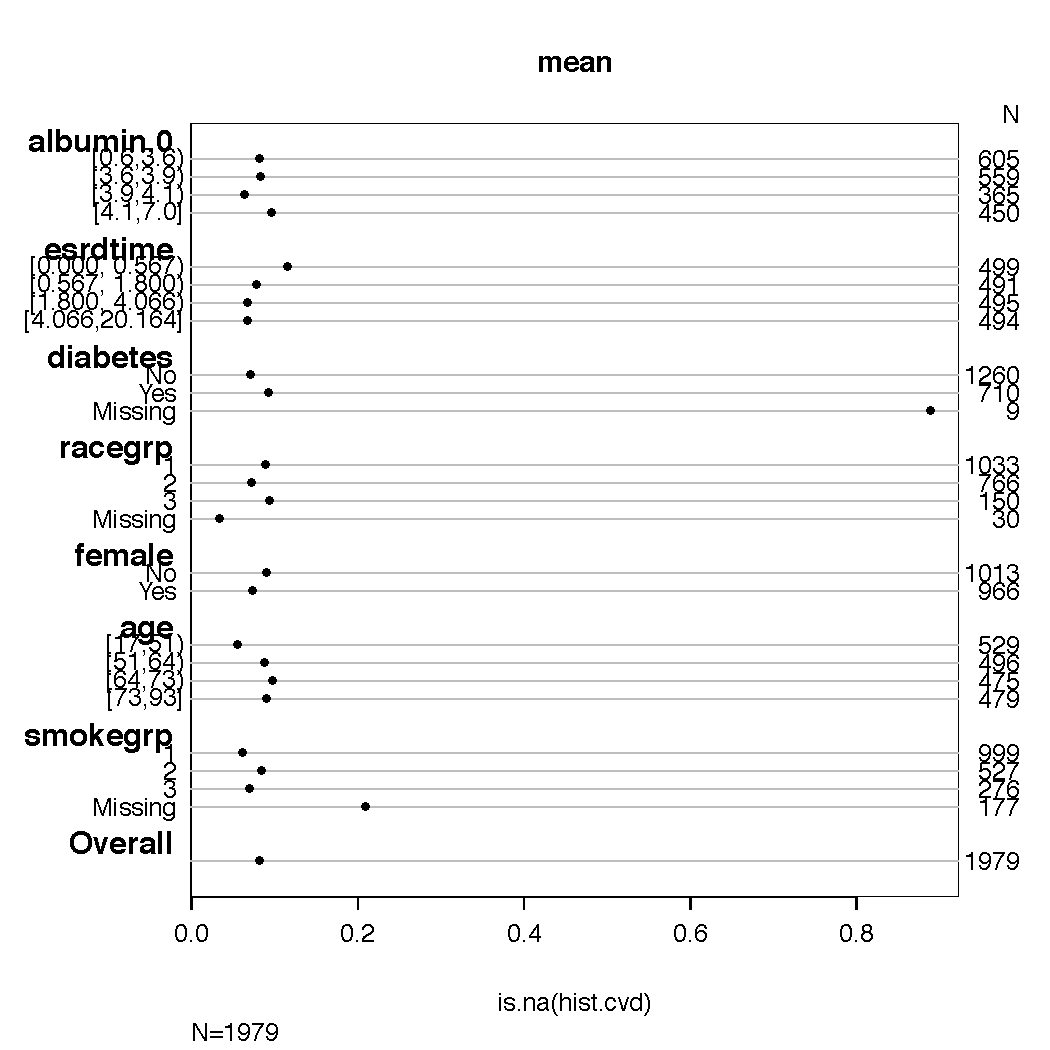
\includegraphics[width=.6\textwidth]{plots/hist_na.pdf}
\caption{Diagram showing patterns of missingness among the history of CVD variable. We note that almost all cases of missing diabetes status also miss information on CVD status. Furthermore, approximately 20\% of subjects that miss CVD status also miss smoking status.}
\label{fig:hist_na}
\end{figure}



\begin{figure}[H]
\centering
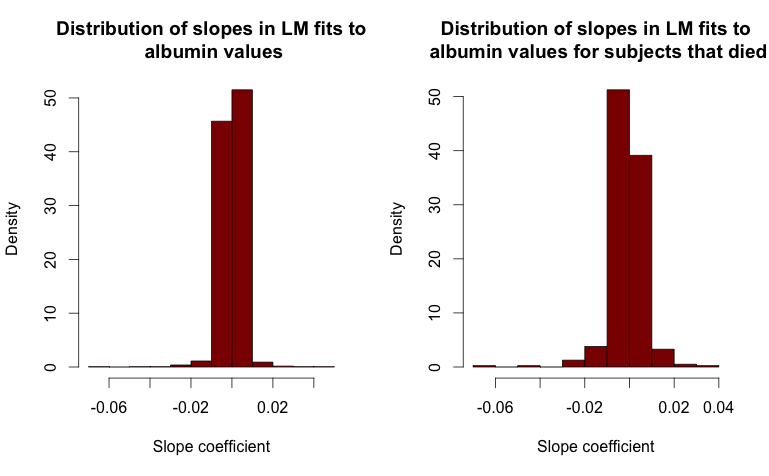
\includegraphics[width=.8\textwidth]{plots/slopes_hist.png}
\label{fig:slopes_hist}
\end{figure}



\section{Fitted Models Supplementary Materials}

\subsection{Model A}

\begin{figure}[H]
\centering
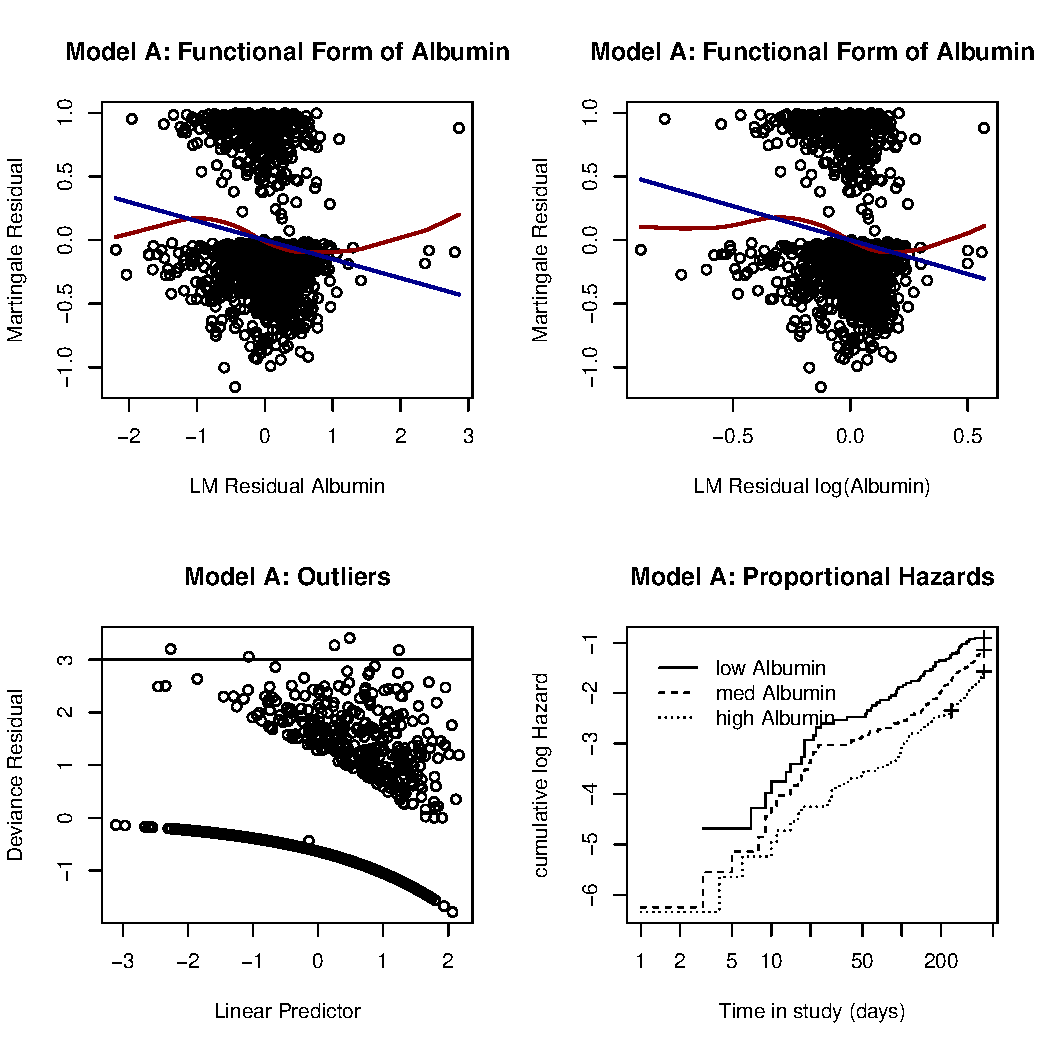
\includegraphics[width=.8\textwidth]{plots/modela_diag.pdf}
\caption{We show a plot of the martingale residuals against the linear model residuals of albumin at recruitment regressed on the other coefficients in the model (top left). We remove the patient with USRDS ID 164447 to obtain a clearer picture of the functional form. The smoother in red seems to be close to the linear line for the spectrum of the points but deviates outside of it. A log transformation of albumin at recruitment (top right) only slightly alleviates this. Setting a cut-off for deviance residuals at -3 and 3 we can see that several points lie just above that line (bottom left). Due to the fact that it is not one single point and there are many points close to this cut-off we do not decide to remove any of the observations. The cumulative log hazards plot (bottom right) seems to show be piecewise parallel.}
\label{fig:modela_diag}
\end{figure}

\begin{figure}[H]
\centering
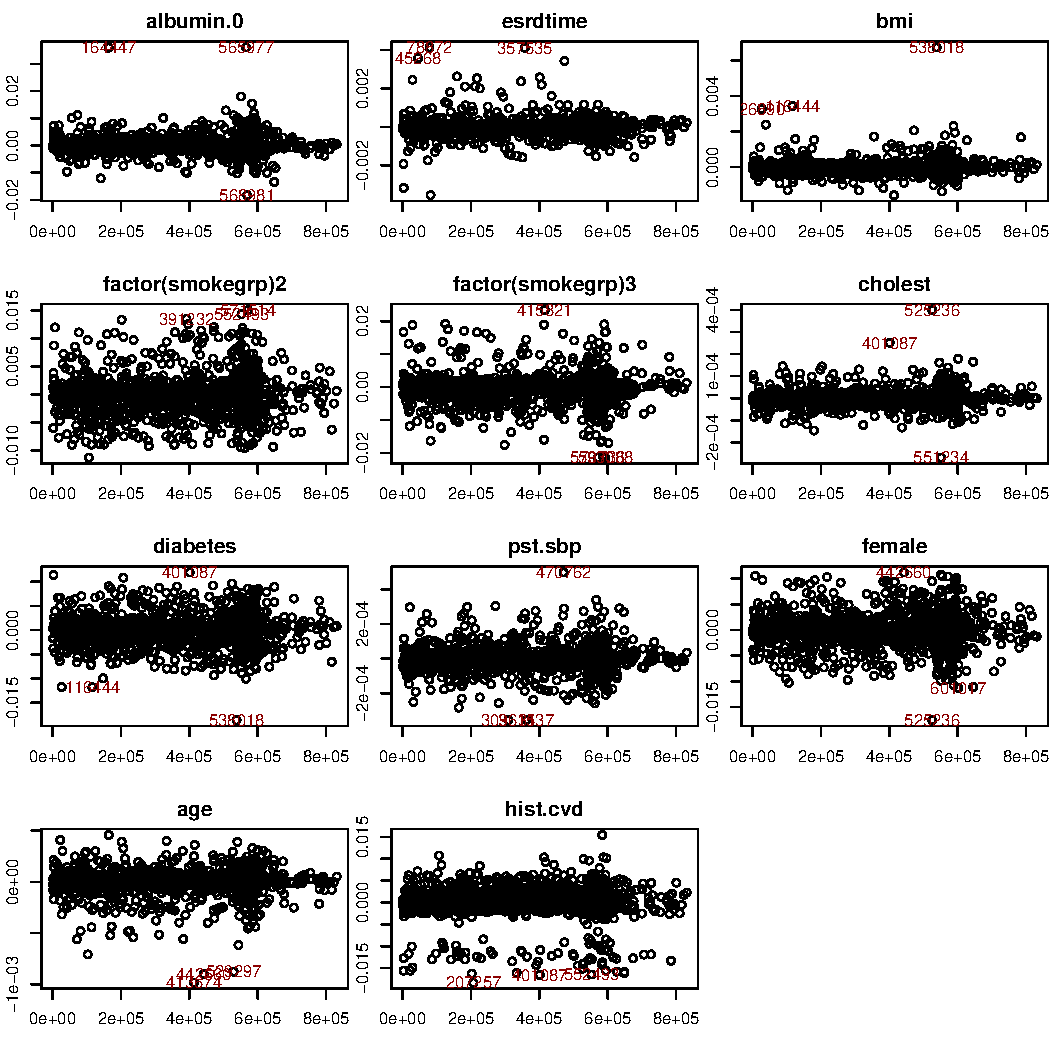
\includegraphics[width=.8\textwidth]{plots/modela_dfbeta.pdf}
\caption{We show plots for the delta beta residuals for each covariate in model A. We indicate patient IDs for the three points with the maximum influence. None of the plots indicates influence of any point higher than of the order of $10^{-2}$. For this reason we decide not to remove any observations.}
\label{fig:modela_dfbeta}
\end{figure}

\subsection{Model B}
\begin{table}[H]
\centering
\begin{tabular}{rll}
  \hline
 & Adjusted relative risk (95\% CI) & p-Value \\ 
  \hline
scale(albumin.0, center = T, scale = F) & 0.37(0.25 ,0.56) & 0 \\ 
  hist.cvd & 2.22(1.67 ,2.94) & 0 \\ 
  esrdtime & 0.99(0.96 ,1.03) & 0.763 \\ 
  bmi & 0.96(0.94 ,0.98) & 0.001 \\ 
  factor(smokegrp)2 & 1(0.78 ,1.29) & 0.984 \\ 
  factor(smokegrp)3 & 1.59(1.16 ,2.16) & 0.003 \\ 
  cholest & 1(1 ,1) & 0.026 \\ 
  diabetes & 1.2(0.95 ,1.5) & 0.12 \\ 
  pst.sbp & 1(0.99 ,1) & 0.092 \\ 
  female & 0.99(0.79 ,1.25) & 0.943 \\ 
  age & 1.04(1.03 ,1.04) & 0 \\ 
  scale(albumin.0, center = T, scale = F):hist.cvd & 1.56(0.98 ,2.49) & 0.058 \\ 
   \hline
\end{tabular}
\caption{Cox model regression estimates of the adjusted relative risk of each patient characteristic for model B. Note that the albumin variable in this model is centered in order to allow for an interpretable interaction.}
\label{tab:model_b}
\end{table}


\begin{figure}[H]
\centering
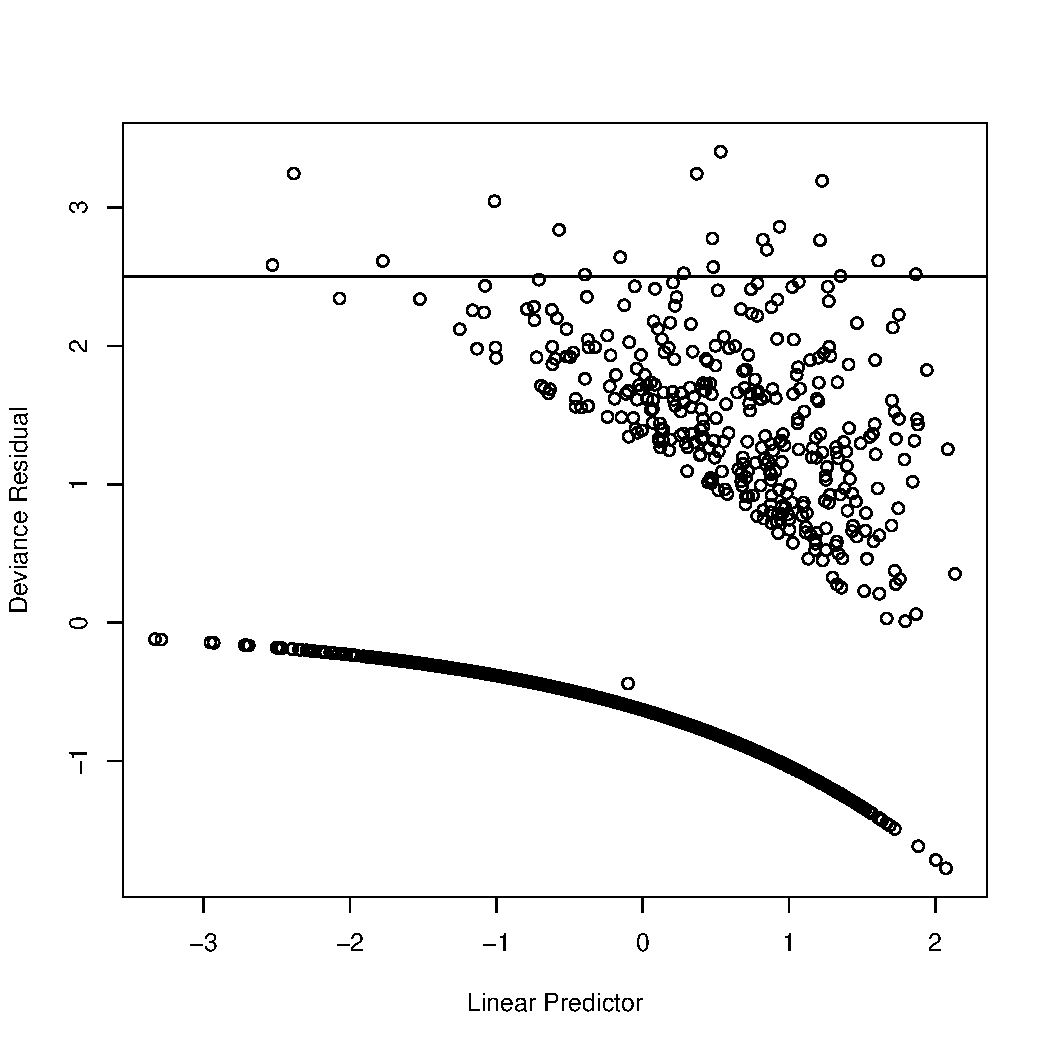
\includegraphics[width=.5\textwidth]{plots/modelb_diag.pdf}
\caption{We show deviance residuals for model B to detect outliers. Similar to model A we have a substanstial number of points that are past the conventional cut-off value of $\pm 3$. However, this cut-off value is not logically significant if many points are over it. We thus decide not to remove any observations.}
\label{fig:modelb_diag}
\end{figure}

\begin{figure}[H]
\centering
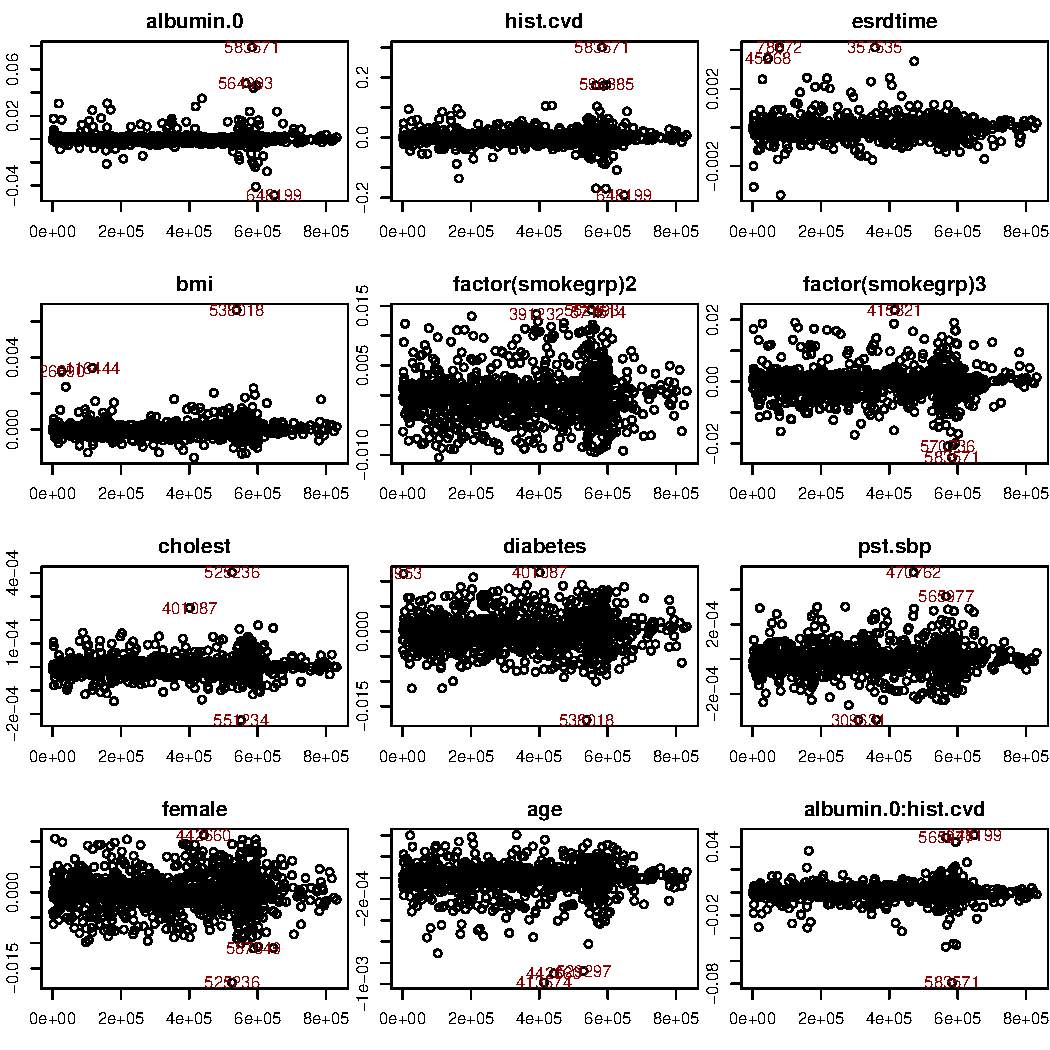
\includegraphics[width=.8\textwidth]{plots/modelb_dfbeta.pdf}
\caption{In these plots we show influence of each observation on each of the covariates in model B. Compared to model A we do have some observations with with influence on the order of $10^{-1}$. We try removing observations with patient IDs 583571, 596385 and 648199. This however hardly changes the estimate for history of CVD. We assume that this is because we have influential points on both the positive and negative side. Thus we decide overall not to remove the observations.}
\label{fig:modelb_dfbeta}
\end{figure}



\subsection{Model C}
\begin{table}[H]
\centering
\begin{tabular}{rll}
  \hline
 & Adjusted relative risk (95\% CI) & p-Value \\ 
  \hline
albumin & 0.48(0.42 ,0.54) & 0 \\ 
  esrdtime & 0.99(0.97 ,1.01) & 0.419 \\ 
  bmi & 0.95(0.94 ,0.97) & 0 \\ 
  factor(smokegrp)2 & 1.1(0.96 ,1.25) & 0.171 \\ 
  factor(smokegrp)3 & 1.63(1.39 ,1.91) & 0 \\ 
  cholest & 1(1 ,1) & 0.033 \\ 
  diabetes & 1.15(1.02 ,1.3) & 0.02 \\ 
  pst.sbp & 1(0.99 ,1) & 0.004 \\ 
  female & 0.98(0.87 ,1.1) & 0.752 \\ 
  age & 1.03(1.03 ,1.04) & 0 \\ 
  hist.cvd & 1.97(1.72 ,2.26) & 0 \\ 
   \hline
\end{tabular}
\caption{Cox model regression estimates of the adjusted relative risk of each patient characteristic for model C. Note that serum albumin is allowed to vary over time. The effect is estimated using the follow up measurements of serum albumin in for patient.}
\label{tab:model_c}
\end{table}

\begin{figure}[H]
\centering
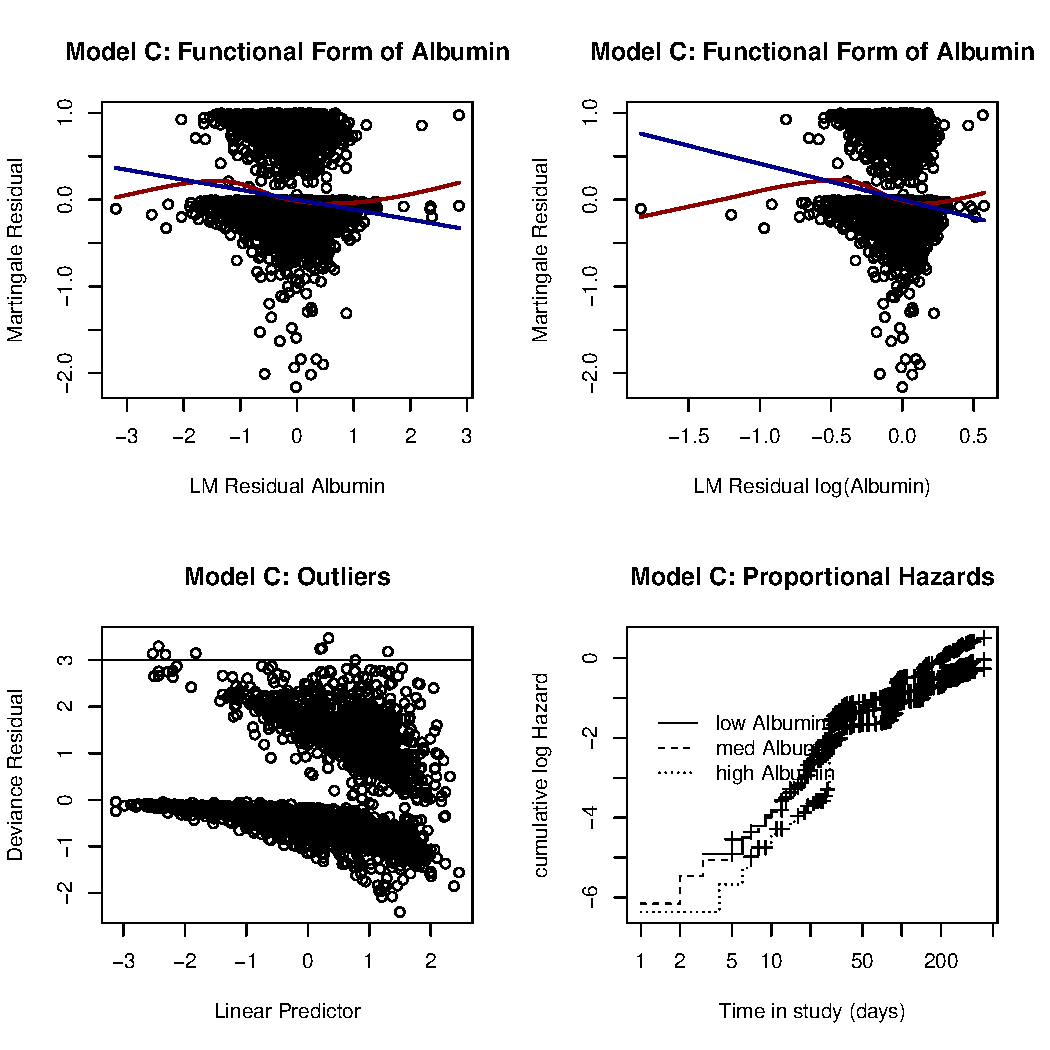
\includegraphics[width=.8\textwidth]{plots/modelc_diag.pdf}
\caption{We show diagnostic plots for model C. The top row shows martingale residual plots for albumin (left) and log(albumin) (right). Similar to the functional form in model A (see figure \ref{fig:modela_diag}) the functional form does not to be exactly linear. However, a log transformation does not seem to drastically improve it. Bottom left shows deviance residuals with the purpose of indicating outliers. As before in model A and B we have many points that fall beyond the conventional $\pm 3$ cut-off. Finally, the log cumulative hazards now seem almost exactly parallel.}
\label{fig:modelc_diag}
\end{figure}

\begin{figure}[H]
\centering
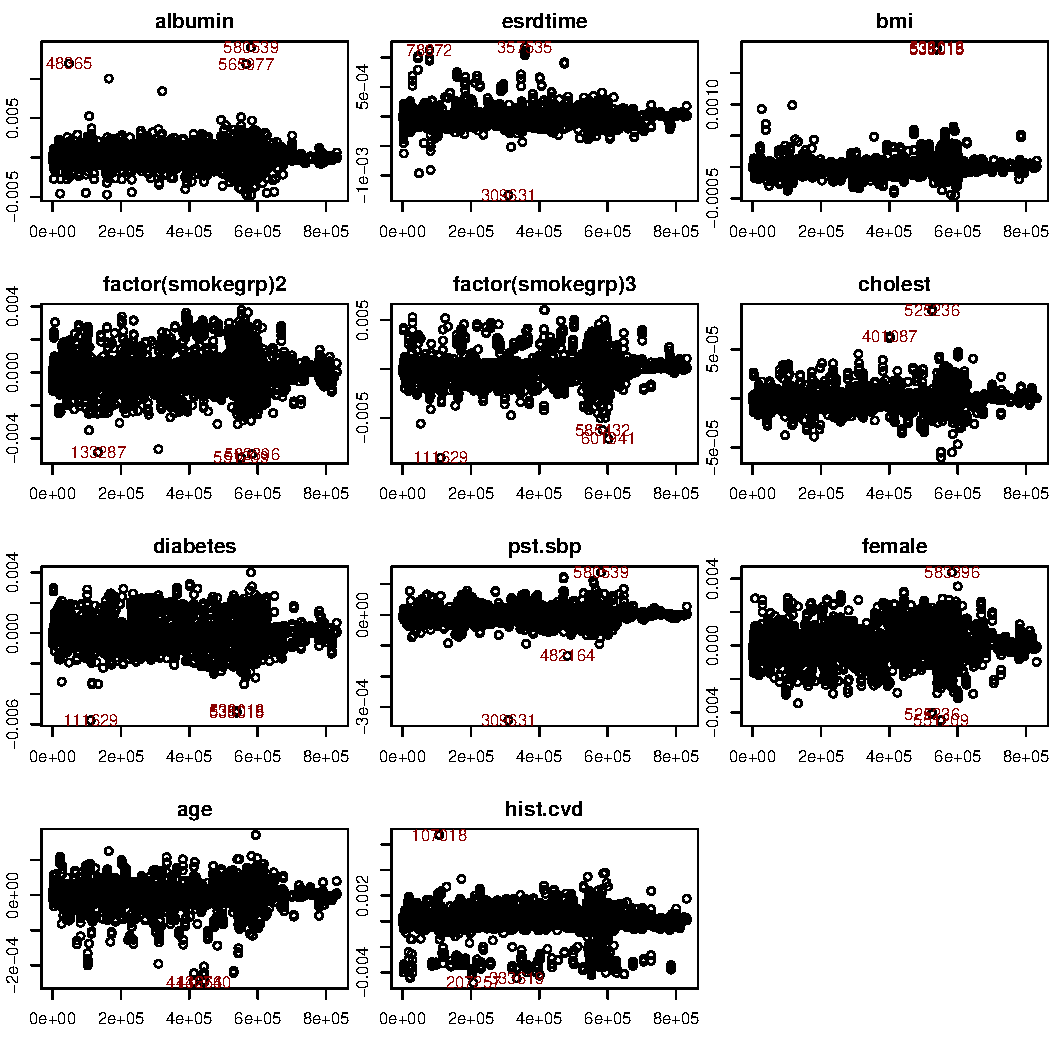
\includegraphics[width=.8\textwidth]{plots/modelc_dfbeta.pdf}
\caption{The plots show delta beta residuals for model C. Each plot thus shows the influence on the respective covariate for each observation. None of the observations have influence higher than of the order of $10^{-3}$. We thus conclude that there are no significantly influential observations for this model.}
\label{fig:modelc_dfbeta}
\end{figure}

\subsection{Model D}
\begin{table}[H]
\centering
\begin{tabular}{rll}
  \hline
 & Adjusted relative risk (95\% CI) & p-Value \\ 
  \hline
scale(albumin, center = T, scale = F) & 0.3(0.24 ,0.38) & 0 \\ 
  hist.cvd & 2.18(1.88 ,2.53) & 0 \\ 
  esrdtime & 0.99(0.98 ,1.01) & 0.584 \\ 
  bmi & 0.95(0.94 ,0.97) & 0 \\ 
  factor(smokegrp)2 & 1.09(0.96 ,1.24) & 0.2 \\ 
  factor(smokegrp)3 & 1.62(1.38 ,1.9) & 0 \\ 
  cholest & 1(1 ,1) & 0.03 \\ 
  diabetes & 1.15(1.03 ,1.3) & 0.018 \\ 
  pst.sbp & 1(0.99 ,1) & 0.007 \\ 
  female & 0.98(0.87 ,1.1) & 0.743 \\ 
  age & 1.03(1.03 ,1.04) & 0 \\ 
  scale(albumin, center = T, scale = F):hist.cvd & 1.82(1.39 ,2.38) & 0 \\ 
   \hline
\end{tabular}
\caption{Cox model regression estimates of the adjusted relative risk of each patient characteristic for model D. This model is equal to model C in all respects apart from that it allows the effect of albumin to vary between patients with and without history of CVD. Note that as in model B we centered the albumin variable.}
\label{tab:model_d}
\end{table}

\subsection{Model E}
\begin{table}[H]
\centering
\begin{tabular}{rll}
  \hline
 & Adjusted relative risk (95\% CI) & p-Value \\ 
  \hline
albumin & 0.54(0.47 ,0.61) & 0 \\ 
  undnour & 1.74(1.53 ,1.98) & 0 \\ 
  esrdtime & 1(0.98 ,1.02) & 0.961 \\ 
  bmi & 0.97(0.96 ,0.98) & 0 \\ 
  factor(smokegrp)2 & 1(0.87 ,1.14) & 0.96 \\ 
  factor(smokegrp)3 & 1.56(1.32 ,1.83) & 0 \\ 
  cholest & 1(1 ,1) & 0.169 \\ 
  diabetes & 1.14(1.01 ,1.29) & 0.031 \\ 
  pst.sbp & 1(0.99 ,1) & 0.001 \\ 
  female & 0.95(0.84 ,1.07) & 0.368 \\ 
  age & 1.03(1.03 ,1.04) & 0 \\ 
  hist.cvd & 2.16(1.87 ,2.5) & 0 \\ 
   \hline
\end{tabular}
\caption{Cox regression coefficients using a time varying serum albumin covariate and adjusting for under nourishment.}
\label{tab:model_e}
\end{table}

\end{document}